\chapter{Previous work}

This project sits at the intersection of two areas of research. 
First there is the application of \Gls{ai} in medical applications, specifically for segmentation problems.
Then, there is the active area of research of \Gls{weaklysupervisedl} machine learning.


Specifically I build strongly upon two existing results:

\begin{enumerate}
    \item The U-Net based approach for building a vertebra instance segmentation model by dr. N. Lessmann et al. \cite{Lessmann2018} based on fully supervised data. This model was developed further in \cite{Chuang2019}
    \item The \acrfull{wise} approach developped by dr. I. Laradji \cite{Laradji2020,Laradji2018}. 
\end{enumerate}

\section{Artificial intelligence for medical applications}

\todo[inline]{Start with short overview of other AI problems (1/2 page)}

\Gls{ai} has proven to be a valuable contribution to medical practice to reduce the burden of repetitive tasks on the medical caregiver.

\todo[inline]{elaborate: ppg to blood pressure - slaapapnue}

\section{Segmentation problems for medical applications}

\todo[inline]{General introduction of U-Net and other medical approaches}

For segmentation tasks, the U-net \cite{Ronneberger2015} is widely used. 
This architecture can be represented by a characteristic U-shape, as the name indicates.
It consists of 

\begin{SCfigure}[][htb]
    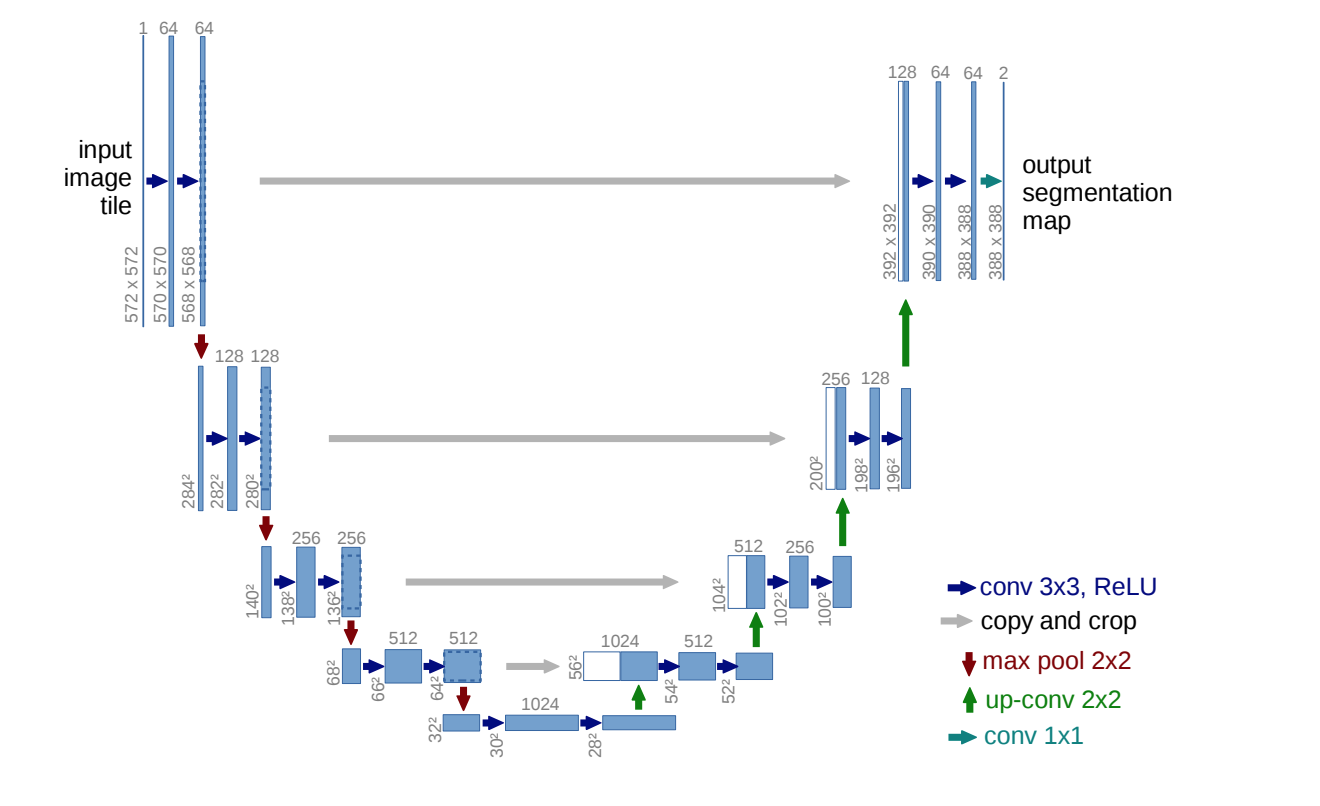
\includegraphics[width=10cm]{/home/thesis/images/UNet_Ronneberger.png}
    \caption{U-Net architecture, as illustrated in \cite{Ronneberger2015}. 
    Each blue box represents a multi-channel feature-map. 
    The number of channels is indicated above the box, the $x \times y$ dimensions are indicated at the bottom left.
    The gray arrows indicate the feature maps in the contracting path are copied and concatenated to the feature maps of the expanding path.}
    \label{fig:unet}
\end{SCfigure}

\todo[inline]{General introduction of U-Net and other medical approaches}

\subsection{Segmentation of the human spine}

\todo[inline]{other authors, approaches --> priors used, metrics used, datasets used}

In this work, the network developed in \cite{Lessmann2018} is used.

\todo[inline]{Concept behind Lessmann, datasets used and results}

\section{Weakly supervised segmentation}




\subsection{General approaches}

\todo[inline]{How is this problem generally solved: PCAMS, WISE, ...}

In this work, the \acrshort{wise} concept is applied for vertebra segmentation.


\begin{SCfigure}[][htb]
    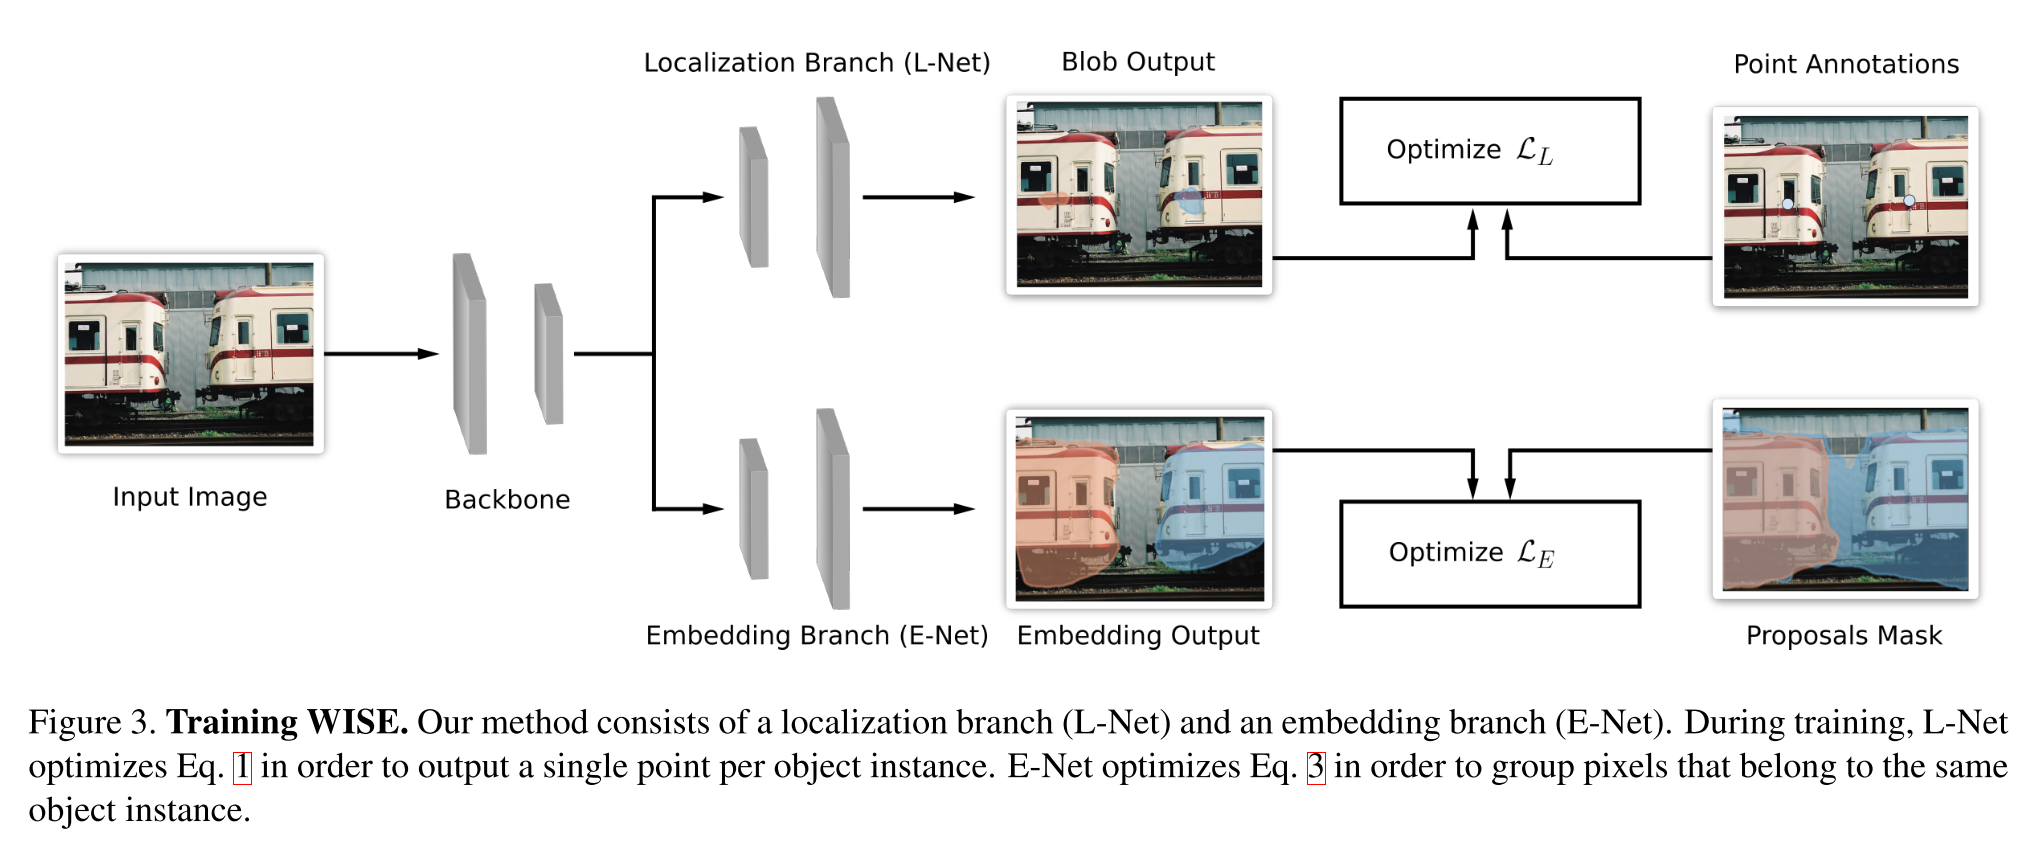
\includegraphics[width=10cm]{/home/thesis/images/Laradji_architecture.png}
    \caption{Illustration from \cite{Laradji2020}. The \acrshort{wise} approach consists of two branches: The Embedding branch and the Localization branch.}
    \label{fig:Laradji}
  \end{SCfigure}

\subsection{Weakly supervised segmentation for Medical applications}

Laradji COVID 19